% Povinný argument: Kód předmětu
\newcommand{\subject}{BPC-PC2M}
% Povinný argument: Název předmětu
\newcommand{\subjectname}{Závěrečný projekt}
% Povinný argument: Seznam autorů
\newcommand{\authors}{Filip Poloček, 240875}
% Povinný argument: Seznam korektorů
%\newcommand{\corrections}{}
% Nepovinný argument: Popis dokumentu
\newcommand{\docdesc}{Game of Life}
% Nepovinný argument: Cílová skupina dokumentu
\newcommand{\docgroup}{}
% Nepovinný argument: URL repozitáře nebo jiný odkaz na dokument
\newcommand{\docurl}{https://github.com/krysar/Game-of-life}

% Přepsáním argumentu na 'false' vypnete balíček 'minted' pro sázení kódu.
% Pro jeho použití lokálně musíte mít v systému dostupný Python 3, python
% knihovnu 'minted' a PDFLaTeX musíte spouštět s argumentem '-shell-escape'.
% Místo něj můžete použít prostředí 'lstlisting'.
\newcommand{\docminted}{true}

% FEKT.tex
% https://github.com/VUT-FEKT-IBE/FEKT.tex
% Git hash repozitáře v době kopírování:

\documentclass[
    % Velikost základního písma je 12 bodů
    12pt,
    % Formát papíru je A4
    a4paper,
    % Jednostranný tisk
    oneside,
    % Záložky a metainformace ve výsledném PDF budou v kódování unicode
    unicode,
]{article}

%%%%%%%%%%%%%%%%%%%%
% OBECNÉ NASTAVENÍ %
%%%%%%%%%%%%%%%%%%%%

% Kódování zdrojových souborů
\usepackage[utf8]{inputenc}
% Kódování výstupního souboru
\usepackage[T1]{fontenc}
% Podpora češtiny
\usepackage[czech]{babel}

% Geometrie stránky
\usepackage[
    % Horní a dolní okraj
    tmargin=25mm,
    bmargin=25mm,
    % Vnitřní a vnější okraj
    lmargin=30mm,
    rmargin=20mm,
    % Velikost zápatí
    footskip=17mm,
    % Vypnutí záhlaví
    nohead,
]{geometry}

% Zajištění kopírovatelnosti a prohledávanosti vytvořených PDF
\usepackage{cmap}
% Podmínky (pro použití v titulní straně)
\usepackage{ifthen}

%%%%%%%%%%%%%%%
% FORMÁTOVÁNÍ %
%%%%%%%%%%%%%%%

% Nastavení stylu nadpisů
\usepackage{sectsty}
% Formátování obsahů
\usepackage{tocloft}
\setcounter{tocdepth}{1}
% Odstranění mezer mezi řádky v seznamech
\usepackage{enumitem}
\setlist{nosep}
\setitemize{leftmargin=1em}
\setenumerate{leftmargin=1.5em}
\renewcommand{\labelitemi}{--}
\renewcommand{\labelitemii}{--}
\renewcommand{\labelitemiii}{--}
\renewcommand{\labelitemiv}{--}
% Sázení správných uvozovek pomocí '\enquote{}'
\usepackage{csquotes}
% Vynucení umístění poznámek pod čarou vespod stránky
\usepackage[bottom]{footmisc}
% Automatické zarovnání textu k předcházení vdov a parchantů
\usepackage[defaultlines=3,all=true]{nowidow}
% Zalomení části textu pokud není na současné stránce dost místa
\usepackage{needspace}
% Nastavení řádkování
\usepackage{setspace}
\onehalfspacing
% Změna odsazení odstavců
\setlength{\parskip}{1em}
\setlength{\parindent}{0em}

% Bezpatkové sázení nadpisů
\allsectionsfont{\sffamily}
% Změna formátování nadpisu a podnadpisů v Obsahu
\renewcommand{\cfttoctitlefont}{\Large\bfseries\sffamily}
\renewcommand{\cftsubsecdotsep}{\cftdotsep}

% Použití moderní/aktualizované sady písem
\usepackage{lmodern}

%%%%%%%%%%%
% NADPISY %
%%%%%%%%%%%

\usepackage{titlesec}

\titlespacing*{\section}{0pt}{10pt}{-0.2\baselineskip}
\titlespacing*{\subsection}{0pt}{0.2\baselineskip}{-0.2\baselineskip}
\titlespacing*{\subsubsection}{0pt}{0.2\baselineskip}{-0.2\baselineskip}
\titlespacing*{\paragraph}{0pt}{0pt}{1em}

%%%%%%%%%%
% ODKAZY %
%%%%%%%%%%

% Tvorba hypertextových odkazů
\usepackage[
    breaklinks=true,
    hypertexnames=false,
]{hyperref}
% Nastavení barvení odkazů
\hypersetup{
    colorlinks,
    citecolor=black,
    filecolor=black,
    linkcolor=black,
    urlcolor=blue
}

%%%%%%%%%%%%%%%%%%%%%%%%%%%
% OBRÁZKY, GRAFY, TABULKY %
%%%%%%%%%%%%%%%%%%%%%%%%%%%

% Vkládání obrázků
\usepackage{graphicx}
\usepackage{subfig}
% Nastavení popisů obrázků, výpisů a tabulek
\usepackage{caption}
\captionsetup{justification=centering}
% Grafy a vektorové obrázky
\usepackage{tikz}
\usetikzlibrary{shapes,arrows}
\usepackage{float}
% Složitější tabulky
\usepackage{tabularx}
\usepackage{multicol}

% Sázení osamocených float prostředí v horní části stránky
\makeatletter
\setlength{\@fptop}{0pt plus 10pt minus 0pt}
\makeatother

% Vynucení vypsání floating prostředí pomocí \FloatBarrier
\usepackage{placeins}

%%%%%%%%%%%%%%
% MATEMATIKA %
%%%%%%%%%%%%%%

% Sázení matematiky a matematických symbolů ('\mathbb{}')
\usepackage{amsmath}
\usepackage{amssymb}
% Sázení fyzikálních veličin
\usepackage{siunitx}

%%%%%%%%%%%%%%%%%
% ZDROJOVÉ KÓDY %
%%%%%%%%%%%%%%%%%

% Sazba zdrojových kódů
\usepackage[formats]{listings}
% Přepnutí prostředí 'code' do režimu výpisu kódu
\newenvironment{code}{\captionsetup{type=listing}}{}

% Balíček 'minted' budeme používat pouze pokud je jeho hodnota nastavena na 'true'
\providecommand{\docminted}{false}
\ifthenelse{\equal{\docminted}{true}}
{
    % Sazba zdrojových kódů
    \usepackage[newfloat]{minted}
    % Nastavení barev 'minted' kódů
    \usemintedstyle{pastie}
}
{
    % \docminted není 'true', nic neprovádíme
    % Pokud je v dokumentu 'minted' prostředí, dokument se nepodaří přeložit.
}

%%%%%%%%%%%
% TITULKA %
%%%%%%%%%%%

\IfFileExists{./.repo.tex}{
    % Soubor '.repo.tex' může (re)definovat povinné a nepovinné argumenty
    % souboru 'main.tex'. To lze využít v případech kdy v jednom repozitáři
    % existuje více dokumentů najednou (např. státnicové otázky).
    \input{.repo}
}{}

% Pokud byly nepovinné argumenty zakomentovány nebo vymazány, přidáme prázdné
% definice příkazů, aby bylo dokument možné správně přeložit.
\providecommand{\docdesc}{}
\providecommand{\docgroup}{}
\providecommand{\docurl}{}

\newcommand{\titulka}{
    \vspace*{2em}
    \begin{center}
        {\Huge \bfseries \subject}

        \vspace*{1em}

        {\Huge \bfseries \subjectname}

        \vspace*{2em}

        {\Large \docdesc}

        \vspace*{1em}

        \docgroup

        \url{\docurl}
    \end{center}

    \vfill

    \begin{tabular}{ll}
        Autor:      & \authors     
    \end{tabular}
    \hfill
    \today

    \thispagestyle{empty}
    \newpage
}


\begin{document}

\titulka{}

\tableofcontents
\thispagestyle{empty}

\setcounter{page}{0}

\newpage

\section{Game of Life}
\label{sec:gol}
Hra života (anglicky \textit{Game of Life}) je dvoustavový celulární automat, který má chováním připomínat společenství živých organismů. Odehrává se na 2D matici buněk.

Buňka může nabývat dvou stavů - je buď mrtvá nebo živá. Její stav v následující generaci je určen stavem jí samotné a jejího Moorova okolí (tj. buněk, se kterými sousedí hranou nebo vrcholem).

Hra života je definována pravidly sestavenými britským matematikem Johnem Conwayem, jež jsou označována jako S23/B3:
\begin{enumerate}
	\item Každá živá buňka s méně než dvěma živými sousedy zemře.
	\item Každá živá buňka se dvěma nebo třemi živými sousedy zůstává žít.
	\item Každá živá buňka s více než třemi živými sousedy zemře.
	\item Každá mrtvá buňka s právě třemi živými sousedy oživne.
\end{enumerate}

\section{Základní popis programu}
\label{sec:zak_pop}
Program načítá výchozí konfiguraci z csv souboru (viz \underline{\hyperref[sec:format]{kapitola 3}}), nechá proběhnout vývoj herního pole po stanovený počet generací a výsledné herní pole uloží do csv souboru ve stejném formátu, jako je vstup. Průběžný vývoj herního pole je vypisován do konzole jedním ze dvou způsobů.
\begin{figure}[H]
	\centering
	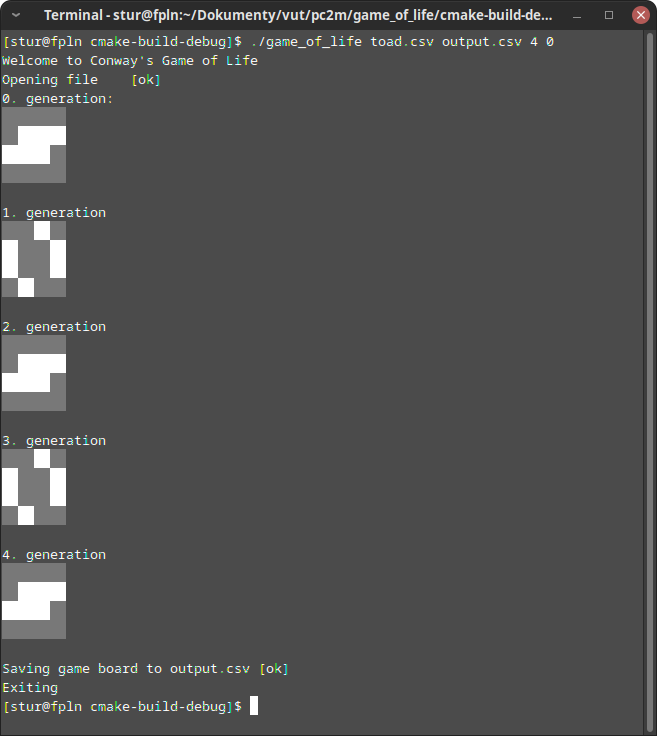
\includegraphics[width=.5\textwidth]{images/toad_run.png}
	\caption{Příklad běhu programu pro 4 generace oscilátoru typu Toad (ropucha)}
	\label{img:1}
\end{figure}

\section{Ovládání}
\label{sec:ovl}
Veškeré parametry jsou programu předávány při spuštění pomocí argumentů příkazového řádku. Syntaxe je následovná:\\
	\texttt{> název{\_}programu [INPUT FILE] [OUTPUT FILE] [GENERATION COUNT] [PRINTING TYPE]}\\
\textbf{Popis parametrů:}\\
\begin{tabular}{l l}
	název{\_}programu & Název spouštěného programu, např. game{\_}of{\_}life.exe \\
	{[INPUT FILE]} & Vstupní csv soubor \\
	{[OUTPUT FILE]} & Výstupní csv soubor \\
	{[GENERATION COUNT]} & Počet generací, po který má hra probíhat. Počáteční je nultá. \\
	{[PRINTING TYPE]} & Formát výpisu do konzole (viz \underline{\hyperref[sec:vypis]{kapitola 5}})
\end{tabular}

\textbf{Příklad:}\\
\texttt{> game{\_}of{\_}life.exe toad.csv output.csv 30 1}

Vzhledem ke způsobu předávání parametrů programu a absenci jakékoliv \textit{zarážky} zabraňující ukončení programu po jeho doběhnutí je nutno program spouštět přímo z prostředí příkazové řádky, nikoliv tedy například rozkliknutí .exe souboru ve správci souborů.

\section{Formát vstupního souboru}
\label{sec:format}
Vstupem je csv soubor, ten definuje počáteční konfiguraci a také velikost herního pole. Jde o tabulku jedniček a nul, jednička je buňka živá, nula buňka mrtvá. Povolený oddělovač sloupců je středník (;) a čárka (,). Velikost herního pole je definována počtem řádků a sloupců tabulky, pole musí být čtvercové (tj. počet sloupců se musí rovnat počtu řádků).

\begin{code}
\centering
\texttt{0;0;0;0\\0;1;1;1\\1;1;1;0\\0;0;0;0}
\caption{Příklad vstupního csv souboru pro oscilátor typu Toad}
\label{code:csv}
Velikost pole je omezena na 255 řádků/sloupců.
\end{code}


\section{Herní pole}
\label{sec:gamefield}
Jak již bylo zmíněno, jde o matici dvoustavových prvků. V programu je implementováno jako dynamicky alokované 2D pole (pointer na pointer) booleanů (datový typ \texttt{bool} z hlavičkového souboru \texttt{stdbool.h}). Jeho alokace probíhá poněkud komplikovaněji v rámci funkce \texttt{read{\_}csv}.

Před počátkem čtení je pole alokováno s velikostí 1x1. Při každém načtení oddělovače sloupců (viz předchozí kapitola) dojde k realokaci s inkrementovaným počtem sloupců, při každém načtení nového řádku pak k realokaci s inkrementovaným počtem řádků. Průběžně probíhá kontrola symetričnosti pole.

Zdrojový kód zde není pro jeho délku začleněn, funkce se nachází v souboru \texttt{gol{\_}csv.c}.

\section{Formát výpisu}
\label{sec:vypis}
Výpis probíhá do \textit{stdout}, což je standardně konzole. Pro správné zobrazení (především u výstupního formátu 1) je nutno zajistit, aby počet řádků konzole odpovídal velikosti herního pole a počet sloupců jeho dvojnásobku.

Posledním vstupním parametrem programu je \texttt{[PRINTING TYPE]} definující druh výpisu, povolené hodnoty jsou 0 a 1.

\subsection{Formát 0}
Tento formát vypíše všechny generace herního pole pod sebe do konzole.

\subsection{Formát 1}
Po každém výpisu herního pole do konzole je zavolán systémový příkaz na její vyčištění (pro Windows \textit{cls}, pro Linux \textit{clear}), díky čemuž je možno relativně názorně sledovat pohyb buněk v poli. Omezením je především rychlost výpisu, u většího herního pole lze narazit na problikávání. Výpis taktéž není nijak bržděn, proto má tenhle formát výpisu smysl jen pro velký počet generací.

Níže je zdrojový kód funkce sloužící k výpisu do konzole, zavolání správného systémového příkazu pro danou platformu je zajištěno podmíněným překladem.
\newpage
\begin{code}
\begin{minted}[frame=lines,framesep=2mm,baselinestretch=1.2,fontsize=\footnotesize,linenos]
{c}
void print_board(bool **field, uint8_t row_count, uint8_t col_count, uint8_t print_type) {
#ifdef _WIN32
    if(print_type == 1)
        system("cls");
    else if(print_type != 0) {
        printf("Error: undefined printing format\n");
        exit(ERR_UNDEFINED_PRINTING);
    }
#elifdef __linux
    if(print_type == 1)
        system("clear");
    else if(print_type != 0) {
        printf("Error: undefined printing format\n");
        exit(ERR_UNDEFINED_PRINTING);
    }
#endif
    for(register uint8_t i = 0; i < row_count; ++i) {
        for(register uint8_t j = 0; j < col_count; ++j) {
            if(field[i][j])
                printf("\u2588\u2588"); // Full block
            else
                printf("\u2591\u2591"); // Light shade
        }
        printf("\n");
    }
    printf("\n");
}
\end{minted}
\caption{Funkce pro výpis herního pole}
\label{code:print_board}
\end{code}
\newpage
Povšimněte si použitých znaků pro pro buňky. Pro živou buňku jsou použity dva znaky \textit{full block}, pro mrtvou dva znaky \textit{light shade}. Nejde o znaky z ASCII, nýbrž z Unicode. Pod Linuxem (a také jinými moderními UN*X systémy) to není problém, standardně se již léta používá znaková sada UTF-8. Pod Windows ovšem nikoliv, je proto ji třeba už na začátku běhu programu manuálně přepnout. Toho jsem docílil podmíněným překladem na začátku funkce main:
\begin{code}
\begin{minted}[frame=lines,framesep=2mm,baselinestretch=1.2,fontsize=\footnotesize,linenos]
{c}
int main(int argc, char *argv[]) {
// On Windows UTF-8 isn't default charset but we're using Unicode characters
#ifdef _WIN32
    system("CHCP 65001");
#endif
...
\end{minted}
\caption{Přepínání znakové sady ve Windows}
\label{code:chcp}
\end{code}

\section{Vývoj herního pole}
\label{sec:vyvoj}
Základní algoritmus pro výpočet následující generace je poměrně jednoduchý a je objasněn v \underline{\hyperref[sec:gol]{první kapitole}}. Taktéž lze vyjádřit tímto vývojovým diagramem:
\begin{figure}[H]
	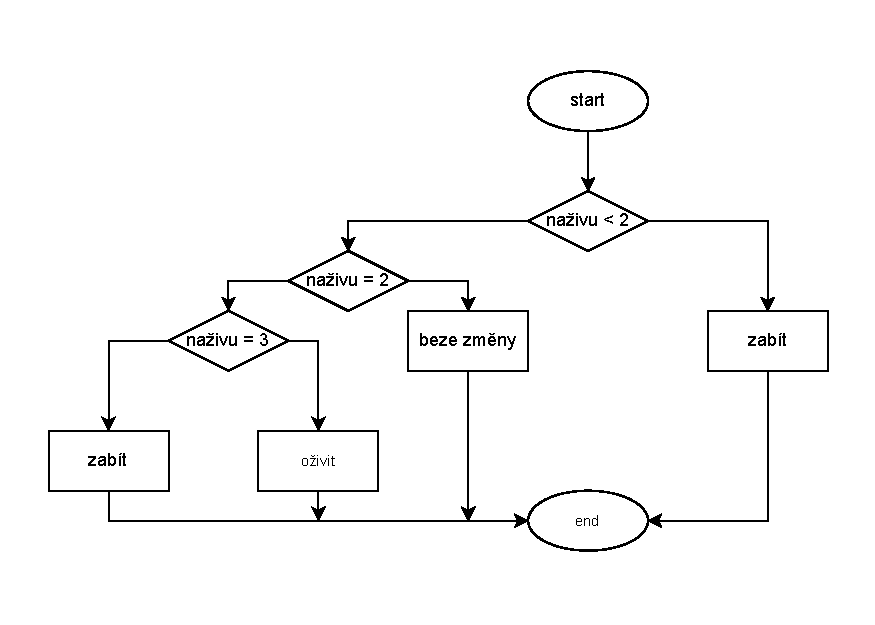
\includegraphics[width=\textwidth]{images/diagram}
	\caption{Diagram vývoje herního pole}
	\label{img:2}
\end{figure}

V rámci programu je algoritmus (s mírným zjednodušením) implementován ve funkci \texttt{update{\_}board} závislé na funkci \texttt{get{\_}num{\_}neighbours} sloužící ke zjištění počtu živých buněk v Moorově okolí zkoumané buňky.

\section{Kompatibilita}
Program je plně kompatibilní s linuxovými distribucemi používající znakovou sadu UTF-8 a se systémem Windows. Částečná kompatibilita je s ostatními UN*X systémy (např. Mac OS), zde není bez doplnění podmíněného překladu možno použít \textit{formát výpisu 1}.

Pro korektní výpis herního pole do konzole je taktéž vhodné, aby počet řádků konzole byl roven velikosti pole a počet sloupců jeho dvojnásobku (čehož lze docílit zmenšením fontu).

\end{document}
